% =====================================================================
%  BTP-1 Report -- Early Prediction of Li-ion Battery Cycle Life
%  IEEE conference format (IEEEtran). Compile with pdfLaTeX + BibTeX
%  (Overleaf default). Section bodies live in sections/*.tex.
% =====================================================================
\documentclass[conference]{IEEEtran}
\IEEEoverridecommandlockouts

\usepackage{cite}
\usepackage{amsmath,amssymb,amsfonts}
\usepackage{graphicx}
\usepackage{booktabs}
\usepackage{array}
\usepackage{multirow}
\usepackage{xcolor}
\usepackage{textcomp}
\usepackage{tikz}
\usetikzlibrary{arrows.meta,positioning,shapes.geometric}
\usepackage[hidelinks]{hyperref}
\usepackage{url}
\usepackage{placeins}  % \FloatBarrier: keep each section's floats near its text

\graphicspath{{figures/}}

% --- helpers ---------------------------------------------------------
\newcommand{\todo}[1]{\textcolor{red}{\textbf{[TODO: #1]}}}
\newcommand{\dq}{\Delta Q_{100-10}(V)}
\newcommand{\Crate}[1]{#1\,C}

\begin{document}

\title{Early Prediction of Lithium-Ion Battery Cycle Life:\\
A Comparative Study of Machine Learning Models\\
and Physics-Informed Features\\[6pt]
\large B.Tech Project (BTP-1) Report}

\author{\IEEEauthorblockN{Samarth Aggarwal}
\IEEEauthorblockA{\textit{Department of Energy Science and Engineering} \\
\textit{Indian Institute of Technology Bombay}\\
Mumbai, India \\
Roll No.\ 23B1502 \quad 23b1502@iitb.ac.in}
\and
\IEEEauthorblockN{Prof. Venkatasailanathan Ramadesigan (Guide)}
\IEEEauthorblockA{\textit{Department of Energy Science and Engineering} \\
\textit{Indian Institute of Technology Bombay}\\
Mumbai, India}
}

\maketitle

\begin{abstract}
Predicting how long a lithium-ion cell will last, using only its first few
charge--discharge cycles, would shorten battery development and validation
from months to days. This project follows the data-driven approach of
Severson \textit{et al.}~\cite{severson2019}. We work with a publicly
released batch of 47 commercial LFP/graphite cells (A123 APR18650M1A,
1.1\,Ah). Each cell was cycled to failure under one of several two-step
fast-charging policies, all of which charge from 0 to 80\% state of charge
in 10 minutes. This interim report documents the experiment and the data.
It describes the conversion of the raw MATLAB files into a Python data
structure and presents an exploratory analysis of capacity fade, internal
resistance, temperature and the discharge voltage curve. Of the 47 cells,
39 have a usable cycle life (392 to 1186 cycles). They fall into two
distinct groups: standard cells (392--514 cycles) and cells marked
\texttt{-newstructure} (777--1186 cycles). The key early-life feature of
\cite{severson2019}, the variance of $\dq$, is strongly correlated with log
cycle life across all cells (Pearson $r=-0.92$). Within each group,
however, the correlation is much weaker ($r=-0.38$ and $r=-0.27$). The
report then sets out the problem statement and the plan for feature
engineering, model training and validation.
The project's main study compares seven machine-learning models (elastic
net, PLS, SVR, Gaussian process, random forest, XGBoost and an MLP) on four
feature sets, from purely data-driven to physics-informed. All models use
one common evaluation protocol and are also tested on an unseen batch.
\end{abstract}

\begin{IEEEkeywords}
lithium-ion battery, cycle life prediction, fast charging, degradation,
machine learning, feature engineering, LFP
\end{IEEEkeywords}

\section{Introduction}
\label{sec:intro}

Measuring the cycle life of a lithium-ion cell means cycling it until its
capacity falls to 80\,\% of nominal, which takes months. Early prediction is
hard because capacity stays nearly flat until a late ``knee'', and because
nominally identical cells differ in life. Severson \textit{et
al.}~\cite{severson2019} predicted cycle life with about 9\,\% error from the
first 100 cycles using features of the discharge curve, chiefly the variance
of $\dq$, the change in the discharge capacity--voltage curve between cycles
10 and 100. This project reproduces that result and asks whether other
model families, features derived from degradation mechanisms or fewer cycles
do better, and how the models transfer to a batch tested differently:
\begin{enumerate}
  \item[\textbf{RQ1}] Using the public data, the paper's train/test split
  and its elastic-net models, do we obtain the test errors of its Table~1
  for feature sets F1--F3 (Table~\ref{tab:featsets})?
  \item[\textbf{RQ2}] With 41 training cells, do non-linear models, a
  Gaussian process (GP) or an additive spline model (GAM), beat the elastic
  net, (a)~for new cells from the training batches and (b)~for a later batch
  tested with a different procedure?
  \item[\textbf{RQ3}] Do features derived from degradation mechanisms
  (dQ/dV peaks, resistance, temperature, anode overhang, capacity budget),
  screened on training cells only, add information beyond $\dq$ and the
  paper's features?
  \item[\textbf{RQ4}] How does the error change when only the first
  $N\in\{20,\dots,150\}$ cycles are used, and what is the smallest useful
  $N$?
  \item[\textbf{RQ5}] Trained only on the three original batches, how
  accurate are the models on an unseen batch with different rests and charge
  termination, and which features cause their errors (SHAP)?
\end{enumerate}

Table~\ref{tab:featsets} defines the 12 features of the paper's sets
F1--F3. The $\Delta Q$ features correlate strongly with life both overall
and within each batch. The temperature integral correlates strongly overall
($-0.70$) but with the opposite sign within each batch, so it mainly
separates the batches; charge time helps only within b1, the one batch in
which it varies.

\begin{table*}[t]
\centering
\caption{The 12 features, all computed from cycles 2--100. $\Delta Q(V)=\dq$
on 1000 voltages from 3.5 to 2.0\,V of the 4\,C discharge; $Q_{d,n}$:
discharge capacity of cycle $n$; $\log=\log_{10}$. Sets: membership in
F1--F3. $r$: Pearson correlation with $\log_{10}$ life on the 41 training
cells (temperature integral: 40, one probe fault), overall and within
batches b1 and b2.}
\label{tab:featsets}
\small
\setlength{\tabcolsep}{3.5pt}
\begin{tabular}{@{}l>{\raggedright\arraybackslash}p{0.43\textwidth}lcccc@{}}
\toprule
Feature & Definition (how it is computed) & Unit & Sets & $r$ & $r_\text{b1}$ & $r_\text{b2}$ \\
\midrule
\multicolumn{7}{@{}l}{\textit{Discharge curve, cycle 100 vs.\ 10}~\cite{severson2019}} \\
$\log\mathrm{Var}\,\Delta Q$ & $\log|\mathrm{Var}_V\,\Delta Q(V)|$, spread of the curve change over voltage & -- & F1 F2 F3 & $-0.90$ & $-0.93$ & $-0.76$ \\
$\log|\min\Delta Q|$ & $\log|\min_V \Delta Q(V)|$, largest local change (on the plateau) & -- & F2 F3 & $-0.89$ & $-0.91$ & $-0.76$ \\
$\log|\mathrm{skew}\,\Delta Q|$ & $\log|$skewness of $\Delta Q(V)$ over $V|$ & -- & F2 & $+0.38$ & $+0.49$ & $-0.22$ \\
$\log|\mathrm{kurt}\,\Delta Q|$ & $\log|$kurtosis of $\Delta Q(V)$ over $V|$ & -- & F2 & $+0.20$ & $+0.63$ & $-0.45$ \\
\midrule
\multicolumn{7}{@{}l}{\textit{Capacity}~\cite{severson2019}} \\
$Q_{d,2}$ & discharge capacity of cycle 2 & Ah & F2 F3 & $+0.33$ & $-0.01$ & $+0.15$ \\
$\max Q_d - Q_{d,2}$ & highest capacity in cycles 2--100 minus $Q_{d,2}$ & Ah & F2 & $+0.15$ & $+0.54$ & $+0.16$ \\
Fade slope & slope $a$ of the least-squares line $Q_{d,n}\approx a\,n+b$, $n=2\dots100$ & Ah/cycle & F3 & $+0.40$ & $+0.46$ & $+0.59$ \\
Fade intercept & intercept $b$ of the same line & Ah & F3 & $+0.28$ & $+0.03$ & $+0.04$ \\
\midrule
\multicolumn{7}{@{}l}{\textit{Other measurements}~\cite{severson2019}} \\
Charge time & mean time from 0 to 80\,\% SOC, cycles 2--6 & min & F3 & $+0.77$ & $+0.77$ & $-0.16$ \\
Temp.\ integral & $\sum_{n=2}^{100}\int T\,dt$ over each cycle (gaps $>10$\,min left out) & $^\circ$C\,min & F3 & $-0.70$ & $+0.06$ & $+0.45$ \\
Min.\ resistance & lowest internal resistance in cycles 2--100 & $\Omega$ & F3 & $-0.39$ & $+0.27$ & $+0.12$ \\
Resistance change & $R_{100}-R_2$ & $\Omega$ & F3 & $+0.38$ & $-0.02$ & $-0.10$ \\
\bottomrule
\end{tabular}
\end{table*}

\section{Background}
\label{sec:background}

\textbf{Test cycle.} The cells are A123 APR18650M1A (LFP/graphite, 1.1\,Ah,
2.0--3.6\,V), cycled at 30\,$^\circ$C~\cite{severson2019}. Each cycle
(Fig.~\ref{fig:cycle}) is a two-step fast charge C1(Q1)--C2 from 0 to
80\,\% SOC in 9--13\,min, a 1\,C charge to 3.6\,V with a constant-voltage
(CV) hold, and a 4\,C discharge to 2.0\,V with a CV hold. How the 3.6\,V hold
ends differs between batches (Section~\ref{sec:dataset}). With age the
overpotential grows: the cell reaches 3.6\,V during the fast charge and the
charger lowers the current (Fig.~\ref{fig:cycle}a). Cycle life is the first
cycle with discharge capacity below 0.88\,Ah (80\,\% of nominal).

\begin{figure}[t]
  \centering
  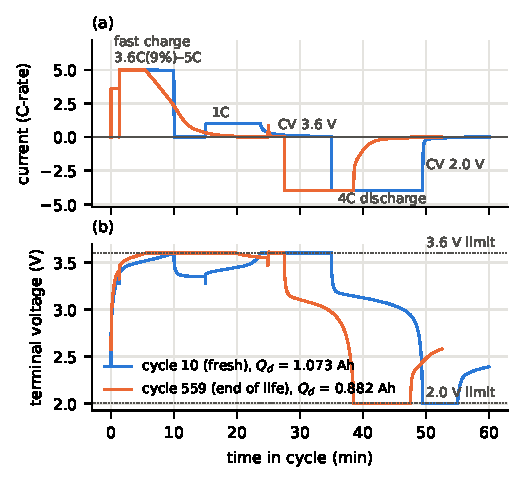
\includegraphics[width=\columnwidth]{fig_cycle}
  \caption{One cycle of cell \texttt{b2c10} when fresh and at end of life.
  (a)~Current; (b)~terminal voltage.}
  \label{fig:cycle}
\end{figure}

\textbf{Degradation.} Because the CV holds let the current decay, the
measured capacity is not limited by resistance; it falls through loss of
lithium (SEI growth, plating) and loss of graphite active material. Loss of
graphite first only shifts the voltage curve, since graphite is in excess.
When its capacity falls below the lithium inventory, lithium plates during
fast charge and the knee follows~\cite{severson2019}. Life is thus set by a
hidden margin that is used up before any capacity loss is visible.

\textbf{What $\dq$ measures.} $\dq=Q_{100}(V)-Q_{10}(V)$ is the horizontal
distance between two 4\,C discharge curves. On the flat LFP plateau a small
change in the curve gives a large shift, so $\dq$ reveals degradation that
the total capacity does not; its variance measures how unevenly the curve
has changed.

\textbf{Anode overhang.} The graphite electrode extends beyond the cathode.
Lithium stored in this overhang returns slowly during the first
cycles~\cite{severson2019}, so capacity first \emph{rises} by a few mAh
(median 3.1\,mAh; 65--80\,\% of it before cycle 10 in b1--b3). Whether the part after cycle 10
carries information is tested in Section~\ref{sec:rq3}.

\section{Dataset and Cleaning}
\label{sec:dataset}

\begin{figure*}[t]
  \centering
  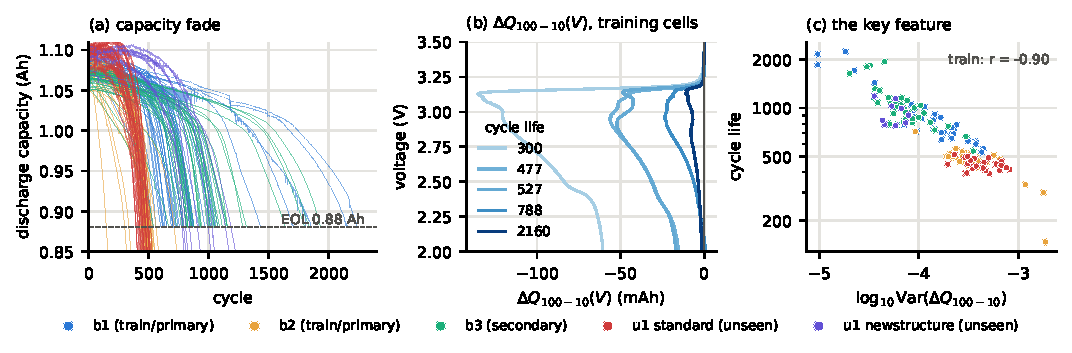
\includegraphics[width=\textwidth]{fig_data}
  \caption{(a) Discharge capacity of all 163 cells. (b) $\dq$ of five
  training cells spanning the life range. (c) Log variance of $\dq$ against
  cycle life for all cells.}
  \label{fig:data}
\end{figure*}

\subsection{Batches and test procedures}
We use the public dataset of~\cite{severson2019,matr_data}: three batches
of the original study (b1--b3, 124 cells, 69 distinct fast-charging policies with
0--80\,\% charge times of 9--13\,min) and a fourth batch from the same
repository, u1 (2018-02-20), which the original study did not use. We keep
the paper's split: 41 training and 43 primary-test cells from b1 and b2, and
the 40 cells of b3 as the secondary test set. u1 has 39 cells with a cycle
life: 30 \emph{standard} cells and 9 marked \texttt{-newstructure}, all
charging to 80\,\% in 10\,min. Its 8 other cells change policy during the
test or were stopped early and have no life label.

Only the fast charge differs between cells, but the rest of the procedure
differs between batches (Table~\ref{tab:batches}), which we measured from
the raw current traces at cycle 50. b3 was also tested about a year after
b1 and b2, so its cells start with less capacity~\cite{severson2019}.

\begin{table}[!htb]
\centering
\caption{Test procedure of each set, measured at cycle 50. Rests: pauses
per cycle; CV end: how the 3.6\,V hold ends; $Q_2$: median capacity at
cycle 2 (Ah); $t_c$: median cycle duration (min).}
\label{tab:batches}
\small
\setlength{\tabcolsep}{3.5pt}
\begin{tabular}{@{}lrccccc@{}}
\toprule
Set & $n$ & Life & Rests & CV end & $Q_2$ & $t_c$ \\
\midrule
b1 & 41 & 534--2237 & 1\,min & time limit & 1.078 & 52 \\
b2 & 43 & 148--713 & 2$\times$5\,min & time limit & 1.072 & 60 \\
b3 & 40 & 541--1935 & 4$\times$5\,s & C/20 & 1.065 & 46 \\
u1 std & 30 & 392--514 & 2$\times$5\,min & C/50 & 1.096 & 69 \\
u1 new & 9 & 777--1186 & 2$\times$10\,s & C/20 & 1.091 & 48 \\
\bottomrule
\end{tabular}
\end{table}

\subsection{Cleaning}
We first apply the cleaning of the authors' code: five b1 cells that never
reached end of life and six faulty b3 channels are dropped, and five b1 cells
that continued in b2 are joined. All 124 cells then match the paper's
Supplementary Table~9 in split, batch and cycle life. Inspecting every batch
showed further faults, fixed by the rules in Table~\ref{tab:cleaning}. Bad
values are set to NaN, never overwritten or invented. Rules C1--C4 affect
0.06\,\% of capacity values and 3.7\,\% of resistance values in cycles
2--100 (the latter almost all from six u1 cells with no resistance record).

\begin{table}[!htb]
\centering
\caption{Cleaning rules added to those of~\cite{severson2019}.}
\label{tab:cleaning}
\small
\setlength{\tabcolsep}{2.5pt}
\begin{tabular}{@{}l>{\raggedright\arraybackslash}p{0.43\columnwidth}>{\raggedright\arraybackslash}p{0.47\columnwidth}@{}}
\toprule
& Fault & Rule \\
\midrule
C1 & Empty first record (b1); resistance $=0$ & set to NaN \\
C2 & Capacity spikes/dips (e.g.\ 2.88\,Ah), test-wide pauses in b2, u1 & $>20$\,mAh from 5-cycle median $\to$ NaN \\
C3 & Corrupt $Q(V)$ curve at glitch cycles & use nearest valid cycle ($\pm2$) \\
C4 & Charge time stuck at 20\,min & set to NaN \\
C5 & Temperature probe off the cell (4 cells) & flag; excluded from F3 \\
C6 & Resistance logger stuck (b1c18, cycles 2--53) & $\ge5$ equal values $\to$ NaN \\
C7 & Time-stamp gaps of hours to days & left out of $\int T\,dt$ \\
\bottomrule
\end{tabular}
\end{table}

\subsection{Exploratory observations}
\label{sec:eda}
\begin{enumerate}
  \item Capacity is nearly flat, or even rises, for most of life and then
  falls at a knee (Fig.~\ref{fig:data}a); lives range from 148 to 2237
  cycles.
  \item $\dq$ is negative mainly on the 3.0--3.2\,V plateau, and its
  magnitude grows with shorter life (Fig.~\ref{fig:data}b). Its log
  variance alone gives $r=-0.90$ with log life on the training cells
  (Fig.~\ref{fig:data}c).
  \item The batches overlap only partly. b2 and u1-standard cells mostly live
  400--550 cycles, b1 and b3 cells much longer. Within u1 the correlation
  is weak ($r=-0.38$ standard, $-0.27$ \texttt{newstructure}), so much of
  the overall trend separates batches and procedures.
  \item Several F3 features mainly encode the procedure. The temperature
  integral tracks cycle duration ($r=0.92$), which is set by the rests
  (Table~\ref{tab:batches}), and the mean charge time varies only within b1.
\end{enumerate}

\section{Methods}
\label{sec:methods}

\subsection{Protocol}
Every model predicts $\log_{10}$(cycle life) from features of cycles $\le N$
(Table~\ref{tab:featsets}). Missing values are filled with the training
median and features are standardised on the training cells. To keep the
small test sets honest, all choices (candidate features, model variants,
settings and the bounds of the GP) are made on the 41 training cells only,
by cross-validation or, where a choice is itself being compared, nested
cross-validation. Each configuration chosen this way is then evaluated once
on the primary and secondary test sets, and all are reported. The unseen
batch u1 is used once, at the end, with every model frozen
(Section~\ref{sec:rq5}). Models using the
temperature integral leave out the four cells with a detached probe, as in
the paper. Randomised steps are repeated with 5--10 seeds; the spread is a few
cycles (at most 11) and is not shown.

\subsection{Metrics}
Predictions of $\log_{10}$ life are converted back to cycles before
scoring. Table~\ref{tab:metrics} lists the scores; RMSE and MAPE are those
of~\cite{severson2019}, the last three are ours.

\begin{table}[!htb]
\centering
\caption{Evaluation metrics. $y_i$, $\hat y_i$: observed and predicted
life of test cell $i$ (cycles).}
\label{tab:metrics}
\small
\setlength{\tabcolsep}{2.5pt}
\begin{tabular}{@{}>{\raggedright\arraybackslash}p{0.20\columnwidth}>{\raggedright\arraybackslash}p{0.42\columnwidth}>{\raggedright\arraybackslash}p{0.34\columnwidth}@{}}
\toprule
Metric & Definition & Purpose / values \\
\midrule
RMSE (cycles) & $\sqrt{\tfrac1n\sum_i(\hat y_i-y_i)^2}$ & typical error; dominated by large errors \\
MAPE (\%) & $\tfrac{100}{n}\sum_i|\hat y_i-y_i|/y_i$ & error relative to life; fair to short-lived cells \\
Constant baseline & every cell predicted at the geometric mean of training lives, 622 cycles (mean of $\log_{10}$ life) & the bar to beat: RMSE 401 (primary), 511 (secondary) \\
In-range RMSE & RMSE over test cells with life in the training range, 300--2160 & separates prediction from extrapolation; drops \texttt{b1c2} (2237) and \texttt{b2c1} (148) \\
Paired bootstrap & RMSE difference of two models on the same resampled test cells; 5000 resamples, 95\,\% interval & difference is real only if the interval excludes 0 \\
GP coverage & share of test cells inside the GP's 95\,\% prediction interval & calibrated if $\approx95$\,\% \\
\bottomrule
\end{tabular}
\end{table}

\subsection{Models}
Table~\ref{tab:models} lists the models; Section~\ref{sec:rq2} explains
the non-linear ones. Trees and neural networks were not among the main
models: a tree cannot predict beyond the training lives, and a neural
network has far more parameters than the 41 cells. One random forest was
tested as a check.

\begin{table}[!htb]
\centering
\caption{Models. All use standardised inputs and predict $\log_{10}$ life;
CV: 4-fold cross-validation repeated 5--10 times on the training cells.}
\label{tab:models}
\small
\setlength{\tabcolsep}{2.5pt}
\begin{tabular}{@{}>{\raggedright\arraybackslash}p{0.14\columnwidth}>{\raggedright\arraybackslash}p{0.46\columnwidth}>{\raggedright\arraybackslash}p{0.35\columnwidth}@{}}
\toprule
Model & Setup & Tuning \\
\midrule
EN~\cite{severson2019} & linear; $\ell_1+\ell_2$ penalty, $\alpha\|w\|_1\rho+\tfrac{\alpha}{2}(1-\rho)\|w\|_2^2$; plain least squares for F1 & $\alpha$ (100 values), $\rho\in[0.1,1]$ (8); CV \\
GP & kernel: linear $+$ Mat\'ern-5/2 (one length-scale per feature) $+$ noise; gives a predictive s.d. & marginal likelihood; length-scale $\ge1$, noise $\ge0.01$ \\
GAM & cubic spline per feature (linear beyond the data) $+$ ridge & knots (3--5), ridge (11); CV \\
RF & 300 trees on bootstrap samples (check only) & leaf size, features per split; CV \\
\bottomrule
\end{tabular}
\end{table}

\subsection{Experiments}
Table~\ref{tab:experiments} lists which models and feature sets answer each
research question. The non-linear models are run on F2 only: it is the
paper's best set on a new batch, while F3 contains batch-dependent features
(Section~\ref{sec:eda}) that already make the elastic net fail on the
secondary batch. No new feature set is used, because none of the screened
candidates added information (Section~\ref{sec:rq3}).

\begin{table}[!htb]
\centering
\caption{Models and feature sets used for each research question. Prim./Sec.:
primary and secondary test sets.}
\label{tab:experiments}
\small
\setlength{\tabcolsep}{2.5pt}
\begin{tabular}{@{}l>{\raggedright\arraybackslash}p{0.58\columnwidth}>{\raggedright\arraybackslash}p{0.27\columnwidth}@{}}
\toprule
RQ & Models $\times$ feature sets & Tested on \\
\midrule
RQ1 & EN on F1 (plain least squares), F2, F3 & Prim., Sec. \\
RQ3 & 19 candidates screened with linear fits; overhang check: EN on F1 and F2 with and without it & Training; Prim., Sec., u1 \\
RQ2 & GP, GAM and a random forest on F2, against EN-F2 & Prim., Sec. \\
RQ4 & EN on F1, F2, F3, recomputed for $N=20$--150 & Prim., Sec. \\
RQ5 & EN on F1, F2, F3; GP, GAM and random forest on F2 & u1 standard and \texttt{newstructure} \\
\bottomrule
\end{tabular}
\end{table}

\section{RQ1: Reproduction of the Paper}
\label{sec:rq1}

The three models of~\cite{severson2019} were rebuilt on F1--F3 with the
protocol of Section~\ref{sec:methods}. The variance model is
$\log_{10}(\text{life}) = 1.346 - 0.396\,\log_{10}\mathrm{Var}(\dq)$. For
the discharge and full models, cross-validation chose an almost ridge-like
penalty ($\rho=0.1$; $\alpha=0.022$ and $0.039$), keeping 6 of 6 and 7 of 9
features.

\begin{table}[!htb]
\centering
\caption{Reproduction of Table~1 of~\cite{severson2019}: ours (paper).
Prim.\ excl.: primary set without \texttt{b2c1}.}
\label{tab:repro}
\small
\setlength{\tabcolsep}{3pt}
\begin{tabular}{@{}lcccc@{}}
\toprule
Model & Train & Primary & Prim.\ excl. & Secondary \\
\midrule
\multicolumn{5}{@{}l}{\textit{RMSE (cycles)}} \\
Constant  & 327 (327) & 401 (401) & 399 (399) & 511 (511) \\
F1 Variance & 104 (103) & 138 (138) & 138 (138) & 196 (196) \\
F2 Discharge & 69 (76) & 90 (91) & 85 (86) & 167 (173) \\
F3 Full & 67 (51) & 125 (118) & 122 (100) & 220 (214) \\
\midrule
\multicolumn{5}{@{}l}{\textit{Mean absolute percentage error (\%)}} \\
Constant  & 29.6 (29.6) & 35.0 (34.9) & 28.2 (28.2) & 36.1 (36.1) \\
F1 Variance & 14.1 (14.1) & 14.7 (14.7) & 13.2 (13.2) & 11.4 (11.4) \\
F2 Discharge & 9.2 (9.8) & 12.6 (13.0) & 9.4 (10.1) & 9.9 (8.6) \\
F3 Full & 6.8 (5.6) & 11.0 (14.1) & 8.0 (7.5) & 11.2 (10.7) \\
\bottomrule
\end{tabular}
\end{table}

\textbf{Results} (Table~\ref{tab:repro}). The constant and variance models match exactly on the test sets. The
discharge model is within 1--6 cycles and the full model within 7 cycles on
both full test sets; the full model's gap is larger on the training set (67 vs.\ 51) and on
the primary set without \texttt{b2c1} (122 vs.\ 100). These gaps are comparable to our own spread over 10 random seeds
(full model: primary 117--128, secondary 218--222 cycles) and are expected
from the paper's different software and sampling. The ranking is the
same, including the paper's key observation that the full model is
\emph{worse} than the discharge model on the secondary set, and the
full-model coefficients agree in sign with the paper's wherever both are
non-zero.

\begin{figure}[!htb]
  \centering
  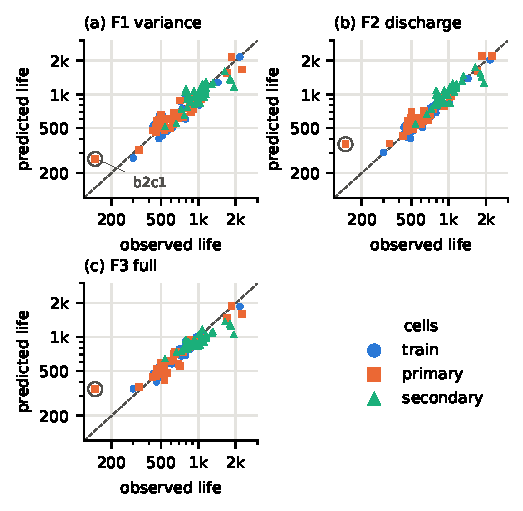
\includegraphics[width=\columnwidth]{fig_rq1_parity}
  \caption{Predicted vs.\ observed cycle life of the three reproduced models
  (log axes; cf.\ Fig.~3 of~\cite{severson2019}). Circled: the anomalous
  cell \texttt{b2c1}.}
  \label{fig:parity}
\end{figure}

\textbf{Where the errors are.} Few training cells live beyond 1500 cycles,
so all three models under-predict the longest-lived cells
(Fig.~\ref{fig:parity}). The longest, \texttt{b1c2} (2237 cycles), is
predicted at 1594 by the full model and alone causes 63\,\% of its squared
error on the primary set. \texttt{b2c1} (148 cycles) is predicted at
266--360; its early failure is not visible in the first 100 cycles.
Within b2 the discharge model is no better than the variance model (MAPE
18.0 vs.\ 17.9\,\% on the primary b2 cells): the skewness and kurtosis of
$\Delta Q$ change sign between b1 and b2 (Table~\ref{tab:featsets}) and get
small weights, so its gain over F1 comes from b1.

\textbf{A data fault.} The first full-model fit predicted 0 cycles for
\texttt{b1c18} (observed 691). In its cycles 2--53 the resistance logger
repeats 19.886\,m$\Omega$ 52 times, and every record contains a time-stamp
jump of 35--67\,h that inflates the temperature integral to 372 standard
deviations above the training mean. Rules C6 and C7
(Table~\ref{tab:cleaning}) fix both, and the prediction becomes 578 cycles.

\textbf{Answer to RQ1.} Yes: the published results are reproduced, exactly
for the variance model and within 7 cycles on the test sets for the others,
with the same ranking.

\section{RQ3: Physics-Informed Features}
\label{sec:rq3}

Nineteen candidates were computed from cycles $\le100$ and screened on the
41 training cells only:
\begin{itemize}
  \item \textbf{Mechanism signatures:} change of the main dQ/dV peak (height,
  voltage, area), charge recovered in the 2.0\,V hold, offset of $\dq$ at
  2\,V, coulombic-efficiency deficit, resistance growth and temperature rise.
  \item \textbf{Shape of the fade:} curvature of the capacity curve, exponent
  of the growth of $\Delta Q_{n-10}(V)$, and a $\dq$ variance averaged over
  several cycles.
  \item \textbf{Policy and procedure:} plating index of the policy,
  temperature at the start of the fast charge, cycle duration.
  \item \textbf{Early capacity rise (anode overhang):} rise before and after
  cycle 10, cycle of the peak, time to half rise.
  \item \textbf{Capacity budget:} \texttt{margin\_rate}, the capacity above
  end of life divided by the degradation rate.
\end{itemize}
A candidate had to add information within each training batch ($t$-statistic
of its coefficient in a linear fit with $\log_{10}\mathrm{Var}(\dq)$), keep
the same sign in b1 and b2, lower the cross-validated error, and still help
on top of a batch label.

\begin{table}[!htb]
\centering
\caption{Screening on the training cells (10 of 19 candidates). $\rho$:
Spearman correlation with $\log_{10}$ life; $t$: $t$-statistic of the
candidate in a linear fit with $\log_{10}\mathrm{Var}(\dq)$, within each batch
($|t|>2.1\approx p<0.05$); Gain: change in CV error when added (\%, positive
= better), alone and on top of a batch label. Bold: passed all criteria.}
\label{tab:screen}
\small
\setlength{\tabcolsep}{2.2pt}
\begin{tabular}{@{}lrrrrr@{}}
\toprule
Candidate & $\rho$ & $t$ b1 & $t$ b2 & Gain & +batch \\
\midrule
dQ/dV peak area change & $+0.77$ & $-1.6$ & $+2.0$ & $-3.6$ & $-2.6$ \\
CV-hold charge at 2.0\,V & $-0.72$ & $+1.9$ & $-2.6$ & $-4.1$ & $-4.7$ \\
Resistance slope vs.\ $\sqrt N$ & $+0.30$ & $+1.8$ & $-2.8$ & $-1.4$ & $+2.7$ \\
Curvature of fade & $+0.53$ & $+2.9$ & $+1.4$ & $-7.4$ & $-5.5$ \\
Exponent of $\Delta Q$ growth & $-0.39$ & $-1.4$ & $+0.6$ & $-0.7$ & $+1.9$ \\
Plating index of policy & $-0.62$ & $+0.8$ & $+2.7$ & $-2.7$ & $+7.6$ \\
Cycle duration & $-0.69$ & $+0.6$ & $-0.7$ & $+24.8$ & $+2.2$ \\
Capacity rise, cycles 2--10 & $+0.20$ & $-2.6$ & $-0.7$ & $+6.4$ & $+3.1$ \\
\textbf{Capacity rise after 10} & $-0.06$ & $-3.9$ & $-1.6$ & $+25.7$ & $+11.2$ \\
\textbf{Margin / rate} & $+0.83$ & $+5.3$ & $+0.1$ & $+9.6$ & $-0.3$ \\
\bottomrule
\end{tabular}
\end{table}

\subsection{Screening results}
\textbf{Mechanism features add nothing.} The dQ/dV, CV-hold, efficiency and
resistance features all increase the cross-validated error
(Table~\ref{tab:screen}). They are computed from the same curves, and $\dq$
already sums the effect of every mechanism.

\textbf{Several features only identify the batch.} Cycle duration lowers the
CV error by 25\,\% on its own but only 2\,\% once the batch is known. The
curvature of the fade correlates with life at $\rho=+0.53$ overall but
$-0.36$ in b1 and $+0.39$ in b2. The plating index of the policy
correlates at $\rho=-0.62$ overall but not within either batch (0.02,
0.03).

\textbf{The fade shows no early acceleration.} In most training cells the
amplitude of $\Delta Q_{n-10}(V)$ grows linearly with $n-10$ (median exponent
1.01, interquartile range 0.98--1.11; Fig.~\ref{fig:rq3}a). The knee cannot be seen in the first 100 cycles,
so curvature and acceleration features carry no extra signal.

\textbf{Two quantities passed the criteria, but neither adds a usable
signal.} (Two timing variants of the overhang rise, the peak and half-rise
cycles, also passed; they carry the same information as
\texttt{overhang\_after10}, $\rho=0.77$--0.89, and are weaker.)
\begin{itemize}
  \item \texttt{margin\_rate}, the capacity left before end of life over the
  degradation rate:
  \begin{align*}
  &\log_{10}\frac{Q_{d,2}-0.88\,\mathrm{Ah}}{\mathrm{sd}(\dq)}\\
  &\quad=\log_{10}(Q_{d,2}-0.88)-\tfrac12\log_{10}\mathrm{Var}(\dq),
  \end{align*}
  and it correlates with $\log_{10}\mathrm{Var}(\dq)$ at $r=-0.995$
  (Fig.~\ref{fig:rq3}b). Its only added information is the initial capacity
  $Q_{d,2}$, which F2 already contains: a free linear fit of
  $\log_{10}\mathrm{Var}(\dq)$ and $Q_{d,2}$ gives the same CV error (0.0635
  vs.\ 0.0649 in $\log_{10}$ life). It is therefore not used.
  \item \texttt{overhang\_after10}, the rise of the 9-cycle rolling median of
  capacity from cycle 10 to its maximum within cycles 2--100
  (Fig.~\ref{fig:rq3}c). Given $\dq$, cells with a
  larger late rise live somewhat shorter ($t=-3.9$ in b1, $-1.6$ in b2;
  Fig.~\ref{fig:rq3}d), consistent with lithium released inside the $\dq$
  window hiding some degradation.
\end{itemize}

\begin{figure}[!htb]
  \centering
  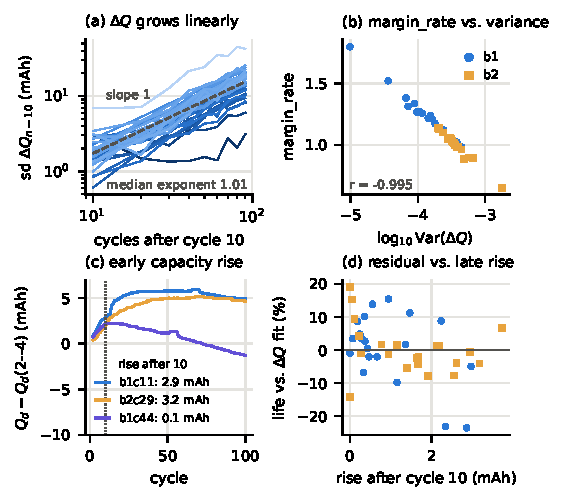
\includegraphics[width=\columnwidth]{fig_rq3_physics}
  \caption{Training cells. (a) Amplitude of $\Delta Q_{n-10}(V)$ (log axes,
  darker = longer life). (b) \texttt{margin\_rate} against
  $\log_{10}\mathrm{Var}(\dq)$. (c) Early capacity of three cells (9-cycle
  rolling median); dotted: cycle 10. (d) Life relative to a $\dq$-only fit
  within each batch, against the rise after cycle 10.}
  \label{fig:rq3}
\end{figure}

\subsection{Does the overhang rise help?}
\texttt{overhang\_after10} was added to F1 and F2 and the elastic net was
evaluated once on all test sets (Table~\ref{tab:overhang}).

\begin{table}[!htb]
\centering
\caption{Elastic net with and without \texttt{overhang\_after10} (OH): CV
error ($\log_{10}$ life, training cells) and test RMSE (cycles). In range:
primary cells inside the training life range.}
\label{tab:overhang}
\small
\setlength{\tabcolsep}{3.5pt}
\begin{tabular}{@{}lccccc@{}}
\toprule
Set & CV & Primary & In range & Secondary & u1 \\
\midrule
F1 & .0717 & 138 & 108 & 196 & 119 \\
F1 + OH & .0536 & 126 & 89 & 205 & 179 \\
\midrule
F2 & .0578 & 90 & 86 & 167 & 260 \\
F2 + OH & .0530 & 113 & 79 & 174 & 189 \\
\bottomrule
\end{tabular}
\end{table}

Within the training batches the rise helps: it lowers the CV error by 25\,\%
on top of F1 and 8\,\% on top of F2, and improves the in-range primary error
(F1: $-19$ cycles, bootstrap interval $-32$ to $-7$; F2: $-7$, $-14$ to $+2$).
On a new batch it does not: on the secondary set both versions are slightly
worse ($+12$ and $+6$, intervals include zero), and on u1 it makes F1
significantly worse ($+60$, $+26$ to $+89$) but F2 better ($-70$, $-93$ to
$-44$). The u1 standard cells have rises of up to 10.8\,mAh against at most
3.7\,mAh in training, so the linear term extrapolates far; with F2 it probably
offsets an over-prediction caused by the capacity features
(Section~\ref{sec:rq5}). An effect that changes sign with the feature set is
not a reliable signal, so the overhang rise is not used either.

\textbf{Answer to RQ3.} No. Mechanism features are redundant with $\dq$,
several candidates only identify the batch, \texttt{margin\_rate} recombines
$\dq$ and $Q_{d,2}$, and the overhang rise helps only within the training
batches. All later sections use F1--F3.

\section{RQ2 and RQ4: Models and Prediction Horizon}
\label{sec:rq2}

\subsection{Non-linear models (RQ2)}
The elastic net assumes that $\log_{10}$ life is linear in the F2 features,
i.e.\ a power law in $\mathrm{Var}(\dq)$ (life $\propto\mathrm{Var}^{-0.40}$
for F1). Section~\ref{sec:rq1} suggests where this may be too simple: the
longest-lived cells are under-predicted, and the skewness and kurtosis of
$\dq$ change sign between b1 and b2, so their effect may depend on other
features. A non-linear model must capture this from 41 cells and still
extrapolate, since some test cells lie outside the training range. Each
model maps the standardised F2 vector $\mathbf z\in\mathbb R^6$ to
$y=\log_{10}$ life.

\textbf{Gaussian process (GP).} The kernel is the linear model plus a
correction:
\begin{equation}
k(\mathbf z,\mathbf z')=\sigma_\ell^2\bigl(\sigma_0^2+\mathbf z^\top\mathbf z'\bigr)
+\sigma_m^2\Bigl(1+\sqrt5\,r+\tfrac53r^2\Bigr)e^{-\sqrt5\,r},
\label{eq:gpkernel}
\end{equation}
with $r^2=\sum_j (z_j-z'_j)^2/\ell_j^2$. The Mat\'ern term gives cells with
similar features similar corrections to the line, which can bend the power
law and couple features; a small length-scale $\ell_j$ makes feature $j$
strongly curved, a large one keeps it linear. With
$A=(K+\sigma_n^2I)^{-1}$ over the training cells and
$\mathbf k_*=k(\mathbf Z,\mathbf z_*)$,
\begin{equation}
\mu(\mathbf z_*)=\mathbf k_*^\top A\,\mathbf y,\quad
s^2(\mathbf z_*)=k(\mathbf z_*,\mathbf z_*)+\sigma_n^2-\mathbf k_*^\top A\,\mathbf k_*.
\end{equation}
Far from the training cells the correction vanishes, so the GP extrapolates
like the elastic net while $s$, and the 95\,\% interval $\mu\pm1.96s$, grow.
Parameters maximise the marginal likelihood; since the unbounded GP
interpolated the 41 cells, $\ell_j\ge1$ and noise variance $\ge0.01$ were
set by nested CV. Fitted, the correction is as large as the linear part
($\sigma_m=0.34$ vs.\ $\sigma_\ell=0.30$), five features sit near the minimum
length-scale, the skewness ($\ell=10^3$) stays linear, and the noise is at
its floor.

\textbf{Additive spline model (GAM).} The GAM lets each feature have its own
curved effect while staying readable:
\begin{equation}
\hat y=\beta_0+\sum_{j=1}^{6}f_j(z_j),\qquad
f_j(z_j)=\sum_{k=1}^{K}\beta_{jk}B_k(z_j),
\end{equation}
with cubic B-splines $B_k$ on equally spaced knots and ridge-penalised
$\beta$. It has no interactions, and beyond the training range each $f_j$
continues linearly with its slope at the edge. CV chose three knots ($K=5$,
30 coefficients for 41 cells) and ridge strength 0.03.

\textbf{Random forest (RF).} Each tree splits the cells by feature thresholds
chosen to minimise
\begin{equation}
\sum_{i:\,z_{ij}\le t}(y_i-\bar y_L)^2+\sum_{i:\,z_{ij}>t}(y_i-\bar y_R)^2
\end{equation}
and predicts the mean of a leaf; 300 bootstrapped trees are averaged. It can
find thresholds and interactions, but cannot predict outside the training
lives (300--2160 cycles). CV chose a minimum leaf of 2 cells and all features
per split.

An RBF support-vector regression (no linear term; \texttt{b1c2} at 1186) and
PLS on the whole $\dq$ curve (secondary RMSE 3431) were also dropped.

\begin{table}[!htb]
\centering
\caption{Non-linear models against the elastic net on F2: test RMSE
(cycles) / MAPE (\%). CV: nested cross-validation RMSE of $\log_{10}$ life
on the training cells. $\Delta$: RMSE change against EN-F2 with 95\,\%
bootstrap interval (negative = better); bold: interval excludes zero.}
\label{tab:rq2}
\footnotesize
\setlength{\tabcolsep}{2.6pt}
\begin{tabular}{@{}lcccc@{}}
\toprule
 & CV & Primary & In range & Secondary \\
\midrule
EN-F2  & \textbf{.0578} & 90 / 12.6 & 86 & \textbf{167} / \textbf{9.9} \\
GP-F2  & .0650 & \textbf{85} / 11.4 & 78 & 174 / 10.5 \\
GAM-F2 & .0776 & 242 / \textbf{10.6} & 79 & 169 / 14.5 \\
RF-F2  & .0951 & 188 / 14.7 & 139 & 226 / 14.5 \\
\midrule
$\Delta$ GP  & & & $-7$\,[$-35$,$+19$] & $+8$\,[$-4$,$+22$] \\
$\Delta$ GAM & & & $-8$\,[$-28$,$+14$] & $+3$\,[$-48$,$+58$] \\
$\Delta$ RF  & & & $+50$\,[$-5$,$+99$] & $\mathbf{+61}$\,[$+26$,$+99$] \\
\bottomrule
\end{tabular}
\end{table}

\textbf{Results} (Table~\ref{tab:rq2}, Fig.~\ref{fig:rq2}). Inside the
training range the GP and the GAM differ from EN-F2 by less than the
bootstrap can resolve, and both have a higher nested-CV error: 41 cells do not
support the extra flexibility. Outside it, the structure decides.
\texttt{b1c2} (2237 cycles) is predicted at 2192 by EN-F2 and 2341 by the GP,
both through their linear term, but at 742 by the GAM, whose curves turn
down near the edge of the data and continue with that slope; the two
out-of-range cells cause 90\,\% of the GAM's squared error. The RF predicts
only between 416 and 1434 cycles (\texttt{b1c2} at 1426, \texttt{b2c1} at
419) and is significantly worse on the secondary batch.

Because it fits the training cells almost exactly (training RMSE 10
cycles), the GP's interval is narrow (typically a factor of 1.16) and covers 81\,\% of the
primary and 95\,\% of the secondary cells; it widens for \texttt{b1c2}
(factor 1.84), which lies far from the training cells.

\begin{figure}[!htb]
  \centering
  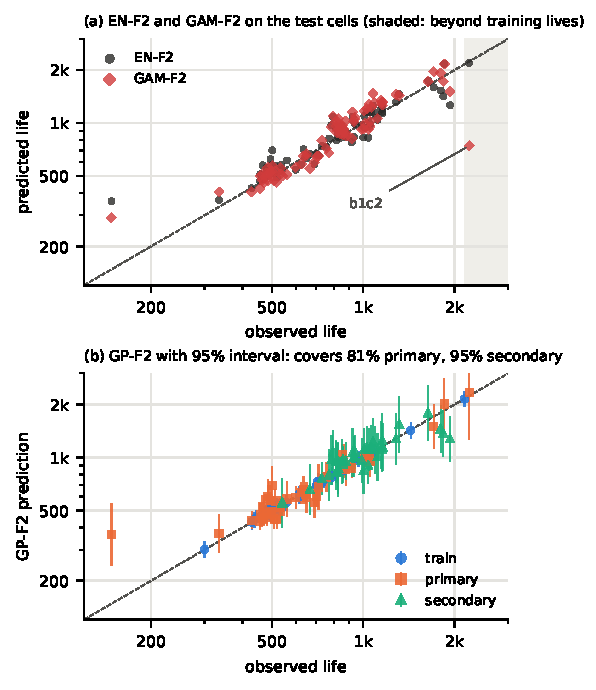
\includegraphics[width=\columnwidth]{fig_rq2_models}
  \caption{(a) EN-F2 and GAM-F2 predictions for the primary and secondary
  test cells. (b) GP-F2 predictions with 95\,\% intervals.}
  \label{fig:rq2}
\end{figure}

\textbf{Answer to RQ2.} No. With 41 training cells neither the GP nor the
GAM is significantly better than the elastic net, within the training
batches or on a new batch; the GAM fails for lives outside the training
range, and the random forest is worse everywhere.

\subsection{Number of early cycles (RQ4)}
All features were recomputed from cycles $\le N$
($\Delta Q_{N-10}(V)$, fits and minima over cycles 2--$N$,
IR($N$)$-$IR(2)) for $N=20$--150, and every model was re-tuned at each $N$.
\texttt{b2c1} (end of life at cycle 148) is excluded from the primary set
at every $N$ (Table~\ref{tab:rq4}, Fig.~\ref{fig:rq4}).

\begin{table}[!htb]
\centering
\caption{Test RMSE (cycles), primary without \texttt{b2c1} / secondary,
against the number of early cycles $N$. Life: median share of a cell's life
used by cycle $N$. F1: least squares. Constant baseline: 399 / 511. Bold:
lowest on each set.}
\label{tab:rq4}
\footnotesize
\setlength{\tabcolsep}{3pt}
\begin{tabular}{@{}rrccc@{}}
\toprule
$N$ & Life & F1 & EN-F2 & EN-F3 \\
\midrule
20  & 3\,\%  & 386 / 475 & 399 / 511 & 233 / 396 \\
30  & 4\,\%  & 324 / 335 & 306 / 350 & 205 / 345 \\
40  & 5\,\%  & 224 / 236 & 191 / 182 & 157 / 212 \\
50  & 7\,\%  & 198 / 258 & 1829 / 1186 & 168 / 247 \\
60  & 8\,\%  & 229 / 234 & 428 / 439 & 142 / 230 \\
80  & 11\,\% & 216 / 213 & 169 / 209 & 146 / 213 \\
100 & 14\,\% & 138 / 196 & 85 / \textbf{167} & 122 / 220 \\
150 & 20\,\% & 122 / 192 & \textbf{82} / 199 & 103 / 224 \\
\bottomrule
\end{tabular}
\end{table}

\begin{figure}[!htb]
  \centering
  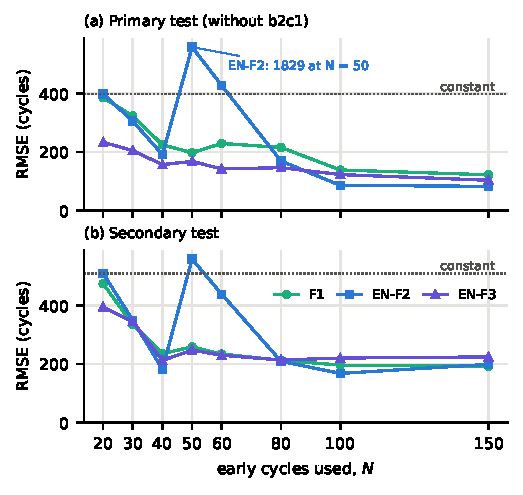
\includegraphics[width=\columnwidth]{fig_rq4_horizon}
  \caption{Test RMSE against the number of early cycles $N$ (values above
  560 clipped). Dotted: constant baseline.}
  \label{fig:rq4}
\end{figure}

\begin{itemize}
  \item \textbf{Up to 30 cycles $\Delta Q$ has no signal.} At $N=20$ the
  elastic net sets every F2 weight to zero and returns the constant, and F1
  is barely better (386 / 475); $\Delta Q_{20-10}$ is mostly noise and
  overhang release. Only F3 does better, through charge time, temperature and
  resistance, which describe the policy and batch rather than the cell; on
  the secondary set its advantage shrinks (396 vs.\ 511).
  \item \textbf{40--80 cycles} (5--11\,\% of life): F1 and EN-F3 reach about
  half the constant-baseline error; EN-F2 does at 40 and 80 cycles but fails
  at 50--60 (last point).
  \item \textbf{80 to 100 cycles: a clear drop} for F1 and F2 (EN-F2 169 to
  85 on the primary set), significant on the secondary set for EN-F2 ($-43$
  cycles). Part of this may be because the features were designed at
  $N=100$.
  \item \textbf{Beyond 100 cycles no gain.} No model improves significantly
  from 100 to 150 cycles.
  \item \textbf{The paper's log-absolute features are fragile early.} At
  $N=50$ EN-F2 predicts 13\,393 cycles for \texttt{b1c0}: its
  $\Delta Q_{50-10}$ is still near zero, so $\log_{10}|\min\Delta Q|$ lies
  8.7 standard deviations outside the training range. F1, which uses only
  the variance, has no such failure (198 / 258).
\end{itemize}

\textbf{Answer to RQ4.} About 40 cycles (5\,\% of life) are enough for a
rough screen at half the baseline error, 100 cycles are clearly better, and
more than 100 bring nothing. Below 30 cycles only policy and batch
information helps.

\section{RQ5: Transfer to an Unseen Batch}
\label{sec:rq5}

The batch u1 is not part of~\cite{severson2019} and was not used for any
choice before this test. Its 39 cells form two groups with different
procedures (Table~\ref{tab:batches}): 30 standard cells with 5-minute rests
and a CV hold to C/50, and 9 \texttt{newstructure} cells with 10-second rests.
Every model was fitted on the 41 training cells with its earlier settings and
applied once. Although the lives (392--1186) lie inside the training range,
the inputs do not: measured against the training cells, the median
$z$-score of the standard cells is $+3.0$ for the temperature integral and
$+2.6$ for $Q_{d,2}$, and that of the \texttt{newstructure} cells is $-1.5$
for $\log_{10}\mathrm{Var}(\dq)$.

\begin{table}[!htb]
\centering
\caption{Frozen models on u1: RMSE (cycles) / mean signed error (\%,
positive = over-prediction).}
\label{tab:rq5}
\footnotesize
\setlength{\tabcolsep}{4pt}
\begin{tabular}{@{}lccc@{}}
\toprule
Model & All (39) & Standard (30) & \texttt{newstructure} (9) \\
\midrule
Constant & 226 / $+22$ & 173 / $+38$ & 351 / $-32$ \\
F1 & \textbf{119} / $+11$ & 77 / $+10$ & \textbf{204} / $+17$ \\
EN-F2 & 260 / $+27$ & 104 / $+20$ & 506 / $+50$ \\
EN-F3 & 138 / $+12$ & \textbf{51} / $+9$ & 271 / $+23$ \\
GP-F2 & 237 / $+26$ & 102 / $+20$ & 458 / $+44$ \\
GAM-F2 & 346 / $+38$ & 183 / $+31$ & 639 / $+62$ \\
RF-F2 & 193 / $+26$ & 113 / $+24$ & 344 / $+34$ \\
\bottomrule
\end{tabular}
\end{table}

\subsection{Results}
\textbf{The standard cells transfer reasonably.} EN-F3 predicts them to
within 51 cycles (9\,\%), F1 to within 77 (14\,\%). These cells resemble b2
in their 5-minute rests and short lives. Within this group the models rank the
cells poorly to moderately (Spearman $\rho=0.19$--0.66).

\textbf{The \texttt{newstructure} cells are over-predicted by every model, by
17--62\,\%.} Their $\dq$ is small, which the models read as a long life
(predictions mostly 1000--1600 cycles), but they live 777--1186 cycles.

\textbf{The ranking differs from the secondary set.} EN-F2, the best model
there, is the worst elastic net here and worse than the constant (260 vs.\
226); EN-F3, the worst there, does well. Over all cells the bootstrap
resolves that F1 beats EN-F2 by 137 cycles (interval 65--201) and EN-F3 beats
EN-F2 by 121 (44--189); F1 and EN-F3 are not resolved ($-17$, $-46$ to
$+20$). The single-feature model is best overall: with fewer features there
is less to extrapolate.

\textbf{Non-linear models do not help.} GP-F2 is slightly better than EN-F2
($-22$, $-42$ to $-3$) but shares its bias; GAM-F2 is the worst model
(346 cycles), over-predicting both groups by 31--62\,\%. RF-F2 beats EN-F2
($-65$, $-107$ to $-16$), but only on the \texttt{newstructure} cells and for
the wrong reason: it cannot predict above about 1430 cycles, which caps the
over-prediction that every model makes there.

\textbf{Uncertainty.} The GP-F2 interval covers 87\,\% of the standard cells
but only 56\,\% of the \texttt{newstructure} cells: it cannot know that the
procedure changed.

\begin{figure}[!htb]
  \centering
  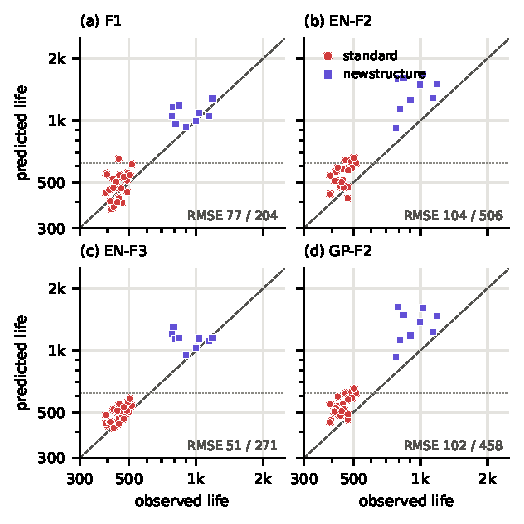
\includegraphics[width=\columnwidth]{fig_rq5_parity}
  \caption{Frozen models on u1 (log axes). RMSE: standard /
  \texttt{newstructure} cells. Dotted: constant baseline (622 cycles).}
  \label{fig:rq5}
\end{figure}

\subsection{Explanation with SHAP}
Exact SHAP values of the predicted $\log_{10}$ life were computed for EN-F2
and EN-F3 with the training cells as background. Fig.~\ref{fig:shap} splits
the mean prediction of each test set into feature contributions and compares
it with the actual mean; the gap is the bias.

\begin{figure}[!htb]
  \centering
  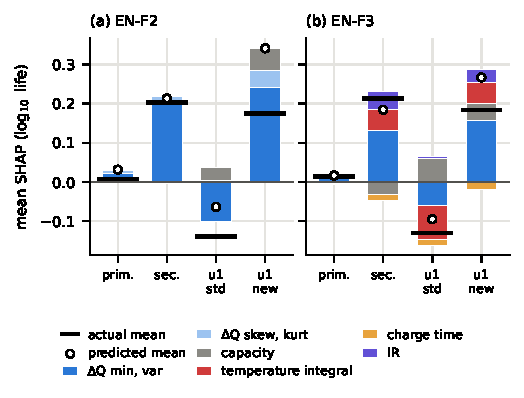
\includegraphics[width=\columnwidth]{fig_rq5_shap}
  \caption{Mean SHAP contribution of each feature group per test set,
  relative to the mean training prediction. Circle: mean prediction; bar:
  actual mean.}
  \label{fig:shap}
\end{figure}

\begin{itemize}
  \item \textbf{EN-F2 over-predicts the standard cells because of their
  capacity.} $\dq$ lowers the prediction ($-0.10$ in $\log_{10}$ life) but
  the high initial capacity raises it ($+0.04$), giving $-0.06$ against an
  actual $-0.14$.
  \item \textbf{EN-F3 is right on the standard cells partly for the wrong
  reason.} Its temperature integral, in effect the long cycle duration,
  lowers the prediction by 0.09 ($\approx-19$\,\%) and cancels the capacity
  effect.
  \item \textbf{The \texttt{newstructure} error comes from $\dq$ itself.}
  The $\dq$ terms add $+0.28$ in EN-F2 against an actual $+0.18$: these cells
  change their discharge curve less than cells of the same life in the other
  batches. No single out-of-range feature is responsible.
\end{itemize}

In EN-F3 the share of the temperature integral rises from 18\,\% of the
attribution on the training cells to 31\,\% on u1, and that of $Q_{d,2}$
from 12 to 23\,\%: the models lean most on the features that lie furthest
outside their training range.

\textbf{Answer to RQ5.} The standard cells, which resemble b2, are
predicted to within 9--14\,\% by EN-F3 and F1; the \texttt{newstructure}
cells are over-predicted by 17--62\,\% by every model because their $\dq$ is
smaller than their life implies. Batch-dependent features help only when the
new batch resembles a training batch, and the simplest model, F1, is the
most robust overall.

\section{Discussion}
\label{sec:discussion}

\textbf{$\dq$ is the signal, and we found nothing to add to it.} Every model
takes most of its information from $\dq$, which already sums the effect of
every mechanism. Over the first 100 cycles it grows linearly, so the early
data contain no sign of the coming knee beyond its rate.

\textbf{The batch, not the model, sets the error.} With two training
batches, anything that separates b1 from b2 looks useful in
cross-validation and on the primary set: the temperature integral and charge
time of F3, the narrow voltage weights of PLS, the extra flexibility of the
GAM, the overhang rise. None of it holds on a new batch. Screening within
each batch (Section~\ref{sec:rq3}) catches part of this, but a model or
feature should finally be judged on a batch it has not seen.

\textbf{The test procedure changes the relation between $\dq$ and life.} In
u1 the \texttt{newstructure} cells live about twice as long as standard
cells charged with the same policy (median 809--997 vs.\ 446--492 cycles for
the three shared policies), and their $\dq$ is smaller still than that longer
life implies.

\textbf{Why b2 and the u1 standard cells live short.} The two short-lived
sets (median 481 and 451 cycles) are the two with 5-minute rests after the
fast charge and after discharge (Table~\ref{tab:batches}; for b2 also stated
in~\cite{severson2019}). The policies do not explain this alone. b2 has only
10-minute policies, but b1 cells with 10-minute policies still live longer
(median 700). 4.8C(80\,\%)-4.8C gives 636--870 cycles in b1 and 461--495 in
b2, and the three policies shared by the two u1 groups give 412--514 cycles
with long rests and 777--1186 with short ones. One policy, 6C(60\,\%)-3C,
barely differs (731--757 in b1, 713 in b2). The end-of-life label is the
same in every batch (first cycle below 0.88\,Ah).

A possible mechanism is temperature: the cell cools during the rests and
starts the fast charge 1.5--2\,\textdegree C colder (31.4--31.6 vs.\
32.8--34.4\,\textdegree C), which favours lithium plating. Within a set and
policy, where the procedure is identical, colder cells do live shorter:
$+6$\,\% life per \textdegree C at the start of the fast charge (95\,\%
interval 4--9\,\%; 112 cells, 36 policy groups). This slope, however,
accounts for only a 9--11\,\% shorter life across the observed temperature
gaps, against 35--55\,\% observed. Temperature contributes, but most of the
effect of the long rests is not explained by the data. Other procedure
differences, such as the CV cut-off, and an unrecorded change behind the
\texttt{newstructure} label cannot be ruled out.

\textbf{Uncertainty needs an out-of-range check.} The GP interval is
too narrow when the GP nearly interpolates the training cells, and
overconfident when the procedure changes (56\,\% coverage on the
\texttt{newstructure} cells). Large input $z$-scores flag some failures, but
not the \texttt{newstructure} cells, whose inputs were only moderately
unusual.

\subsection{Limitations}
\begin{itemize}
  \item \textbf{Small sample.} 41 training cells and about 40 cells per test
  set: most differences between models have bootstrap intervals that include
  zero. Many configurations were scored on the same test sets; fixing every choice on the training cells
  and the bootstrap limit, but do not remove, the optimism this causes.
  \item \textbf{Narrow scope.} One cell type (LFP/graphite, A123), one
  temperature (30\,\textdegree C), two training batches and only nine
  \texttt{newstructure} cells.
  \item \textbf{Limited search.} Nineteen candidates were screened; other
  features (e.g.\ from the charge curve or relaxation voltage) were not
  tried.
  \item \textbf{Unlabelled procedure changes.} What \texttt{newstructure}
  changes is inferred from the step records (rests, CV cut-off); other
  changes cannot be ruled out.
  \item \textbf{Two-cycle features.} $\dq$ uses only cycles 10 and 100, so
  noise in either passes directly into every feature.
\end{itemize}

\section{Conclusion}
\label{sec:conclusion}
The data-driven early prediction of~\cite{severson2019} was reproduced on a
cleaned pipeline, exactly for the one-feature model and within a few cycles
for the others (RQ1). Nineteen features derived from degradation mechanisms
were screened, and none added usable information beyond $\dq$ and the
paper's capacity features (RQ3). With 41 training cells, a Gaussian process
and an additive spline model were not significantly better than the
elastic net, within the training batches or on a new batch; the spline
model fails beyond the training range, and a random forest, which cannot
extrapolate at all, is worse everywhere (RQ2). About 40 cycles give a rough
prediction, 100 cycles a good one, and more bring no gain (RQ4). On an
unseen batch, cells tested like a training batch are predicted to within
9--14\,\%, while cells tested with a different procedure are over-predicted
by 17--62\,\% by every model; SHAP traces this to $\dq$ itself (RQ5). The
main obstacle to early life prediction on this dataset is the change of test
procedure between batches, not the choice of model or features.

\textbf{Future work.}
\begin{itemize}
  \item Train on more batches and procedures, including u1, and evaluate
  leave-one-batch-out.
  \item Give the model the procedure (rest length, CV cut-off) as an input,
  or correct $\dq$ for it.
  \item Fit $\dq$ over all cycles 10--100 instead of two, using its linear
  growth, to reduce noise.
  \item Combine the GP interval with an out-of-range check before trusting a
  prediction.
  \item Look for new information in signals not used here, such as the
  charge curve or rest voltage relaxation, and test on other chemistries and
  in closed-loop protocol optimisation~\cite{attia2020}.
\end{itemize}


\bibliographystyle{IEEEtran}
\bibliography{refs}

\end{document}
